%% arara directives
% arara: xelatex
% arara: bibtex


%\documentclass{article} % One-column default
\RequirePackage[2020-02-02]{latexrelease}
\documentclass[twocolumn, switch]{article} % Method A for two-column formatting

\usepackage{preprint}

%% Math packages
\usepackage{amsmath, amsthm, amssymb, amsfonts}

%% Algorithm packages
\usepackage{algorithm}
\usepackage{algpseudocode}
% Images width
\newcommand\x{0.7}
%% Bibliography options
\usepackage[numbers,square]{natbib}
\bibliographystyle{unsrtnat}
%\usepackage{natbib}
%\bibliographystyle{Geology}

%% General packages
\usepackage[utf8]{inputenc}	% allow utf-8 input
\usepackage[T1]{fontenc}	% use 8-bit T1 fonts
\usepackage{xcolor}		% colors for hyperlinks
\usepackage{graphicx}
\graphicspath{{./assets/}}
\usepackage[colorlinks = true,
            linkcolor = purple,
            urlcolor  = blue,
            citecolor = black,
			allcolors = black,
            anchorcolor = black]{hyperref}	% Color links to references, figures, etc.
\usepackage{booktabs} 		% professional-quality tables
\usepackage{nicefrac}		% compact symbols for 1/2, etc.
\usepackage{microtype}		% microtypography
\usepackage{lineno}		% Line numbers
\usepackage{float}			% Allows for figures within multicol
%\usepackage{multicol}		% Multiple columns (Method B)

\usepackage{lipsum}		%  Filler text

 %% Special figure caption options
\usepackage{newfloat}
\DeclareFloatingEnvironment[name={Supplementary Figure}]{suppfigure}
\usepackage{sidecap}
\sidecaptionvpos{figure}{c}

% Section title spacing  options
%\usepackage{titlesec}
%\titlespacing\section{0pt}{12pt plus 3pt minus 3pt}{1pt plus 1pt minus 1pt}
%\titlespacing\subsection{0pt}{10pt plus 3pt minus 3pt}{1pt plus 1pt minus 1pt}
%\titlespacing\subsubsection{0pt}{8pt plus 3pt minus 3pt}{1pt plus 1pt minus 1pt}
\usepackage[compact]{titlesec}
\titlespacing{\section}{0pt}{*0}{*0}
\titlespacing{\subsection}{0pt}{*0}{*0}
\titlespacing{\subsubsection}{0pt}{*0}{*0}

% ORCiD insertion
\usepackage{tikz,xcolor,hyperref}

\definecolor{lime}{HTML}{A6CE39}
\DeclareRobustCommand{\orcidicon}{
	\begin{tikzpicture}
	\draw[lime, fill=lime] (0,0) 
	circle [radius=0.16] 
	node[white] {{\fontfamily{qag}\selectfont \tiny ID}};
	\draw[white, fill=white] (-0.0625,0.095) 
	circle [radius=0.007];
	\end{tikzpicture}
	\hspace{-2mm}
}
\foreach \x in {A, ..., Z}{\expandafter\xdef\csname orcid\x\endcsname{\noexpand\href{https://orcid.org/\csname orcidauthor\x\endcsname}
			{\noexpand\orcidicon}}
}
% Define the ORCID iD command for each author separately. Here done for two authors.
\newcommand{\orcidauthorA}{0000-0000-0000-0001}
\newcommand{\orcidauthorB}{0000-0000-0000-0002}
\newcommand{\orcidauthorC}{0000-0000-0000-0003}
\newcommand{\orcidauthorD}{0000-0000-0000-0004}

%%%%%%%%%%%%%%%%   Title   %%%%%%%%%%%%%%%%
\title{Machine Learning techniques for malicious PDF detection}

% Add watermark with submission status
\usepackage{xwatermark}
% Left watermark
% \newwatermark[firstpage,color=gray!60,angle=90,scale=0.32, xpos=-4.05in,ypos=0]{\href{https://doi.org/}{\color{gray}{Publication doi}}}
% Right watermark
% \newwatermark[firstpage,color=gray!60,angle=90,scale=0.32, xpos=3.9in,ypos=0]% {\href{https://doi.org/}{\color{gray}{Preprint doi}}}
% Bottom watermark
% \newwatermark[firstpage,color=gray!90,angle=0,scale=0.28, xpos=0in,ypos=-5in]% {*correspondence: \texttt{email@institution.edu}}
%%%%%%%%%%%%%%%  AUTHORS LIST  %%%%%%%%%%%%%%%
\usepackage{authblk}
\renewcommand*{\Authfont}{\bfseries}
\author{Lorenzo Ippolito, Mattia Rosso, Martino Picasso}


%%%%%%%%%%%%%%    Front matter    %%%%%%%%%%%%%%
\begin{document}

\twocolumn[ % Method A for two-column formatting
	\begin{@twocolumnfalse} % Method A for two-column formatting

		\maketitle
		%%%# ABSTRACT #%%
		\begin{abstract}
			This project presents an exaustive analysis of machine learning techniques for detecting malicious PDF files. By comparing the performance of four binary classification models - Support Vector Machines (SVM), K-Nearest Neighbors (KNN), Decision Trees and Random Forests - we demonstrate the effectiveness of these approaches in achieving high accuracy and low false negative rates.
			What makes this project stand out is its focus on the machine learning models themselves, including the careful selection of hyperparameters to optimize their performance. Additionally, the inclusion of KNN as a valid model is rare in the field, and the analysis of evasion techniques adds another layer of depth to the study. Overall this paper, realized for the MALIS course at EURECOM (year 2022/2023), offers a comprehensive look at the use of machine learning for malicious PDF detection and the potential vulnerabilities of these models.
		\end{abstract}
		%\keywords{First keyword \and Second keyword \and More} % (optional)
		\vspace{0.35cm}

	\end{@twocolumnfalse} % Method A for two-column formatting
] % Method A for two-column formatting

%\begin{multicols}{2} % Method B for two-column formatting (doesn't play well with line numbers), comment out if using method A


%%%%%%%%%%%%%%%  Main text   %%%%%%%%%%%%%%%
% \linenumbers

%%%# INTRODUCTION #%%
\section{Introduction}
PDF (Portable Document Format) is a file format used for exchanging and sharing documents. It can contain various types of elements, such as text, images, multimedia, and executable code. Keywords, also known as actions or triggers, specify the different types of contents and they can be used to detect whether the file is malicious or Benign. In addition, PDF files may include also fonts, annotations, and form fields, which can be exploited for malicious purposes. We implemented four different binary classifiers to analyze their performances and to prove which one achieves the best results in terms of Accuracy and False Negative Rate. The task is a binary classification, with malicious PDFs labelled as Positive and Benign PDFs labelled as Negative. We also investigated evasion techniques against our classifiers concluding the work with the implementation of a countermeasure algorithm known as Adversarial Learning.


%%# RELATED WORK #%%
\section{Related work}
\label{sec:relatedwork}
Most of the publications on this topic makes use of the Contagio dataset \cite{Contagio} that is the one we have adopted as benchmark. We have considered some of them. Maiorca et al. \cite{maiorca_giacinto_corona_1970} preprocesses data with PDFiD \cite{PDFiD} and uses SVM and Random Forest,  Cuan et al. \cite{cuan_damien_delaplace_valois_2018} uses both PDFiD as preprocessing and train a RBF SVM, they also explain how to perform evasion attacks and relative countermeasures. In \cite{li_liu_yan_yang_2022} Li et al. explain the iterative Gradient Descent attack algorithm against RBF SVM.

%%# DATASETS AND FEATURES #%%
\section{Datasets and features}
\label{sec:datasetsandfeatures}
As first step in building our model, we needed to obtain a dataset of PDFs to use for training and evaluation and we went for the Contagio dataset. It is a collection of malicious PDF files that has been widely used for research and testing purposes. The dataset contains about 20000 PDF samples (almost balanced between Malicious and Benign), including malware, phishing attacks, and other types of malicious contents. The samples in the dataset are representative of the types of threats that are commonly encountered.\newline
We chose to perform a static analysis, which does not require opening the PDFs in a reader. Indeed, we used a tool called PDFiD to extract relevant information from the PDFs. PDFiD characterizes each PDF by extracting the number of occurrences of specific keywords. This allowed us to map each PDF into an array of 21 elements that became our features vector.\newline
Among the keywords that we selected, some are related to the structure of the PDF file, such as \textit{obj} and \textit{endobj}, which mark the beginning and end of an object, \textit{stream} and \textit{endstream}, which mark the beginning and end of a stream of data. We also included \textit{xref}, \textit{trailer}, and \textit{startxref}, which pertain to the organization of the file. Next, there are features related to the content of the PDF: we added \textit{/Page}, which specifies a page object in the file, and \textit{/Encrypt}. We also included \textit{/ObjStm}, which denotes an object stream, \textit{/JS} and \textit{/JavaScript}, which indicate the presence of JavaScript code. Additionally, we selected features related to actions that can be triggered by the PDF, such as \textit{/AA}, \textit{/OpenAction}, \textit{/XFA} and \textit{/AcroForm}, that could potentially exfiltrate information from users. We also included the features related to the types of data that may be present in the file, such as \textit{/JBIG2Decode}, \textit{/RichMedia}, \textit{/Launch} and \textit{/EmbeddedFile}. Finally we also chose \textit{/Colors}, which specifies the presence of more than 16 million colors.\newline
The output of PDFiD is then converted into a CSV file, which can be easily accessed using the \texttt{numpy} and \texttt{pandas} Python libraries. This CSV file serves as the basis for our data extraction pipeline, which we have implemented using the functions provided by PDFiD. It is important to note that the keywords we selected are well known to be discriminant for PDF malware analysis but they do not represent the full set that may appear in a PDF file.\newline
The plot in Figure \ref{fig:parallel} shows that the features distribution is much different between Benign and Malicious PDFs.

\begin{figure}[ht!]
	\centering
	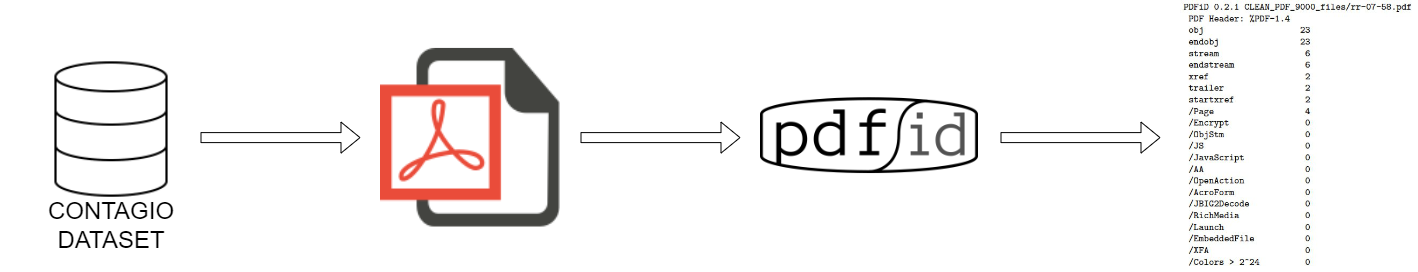
\includegraphics[width=\x\linewidth]{data_extraction.png}
	\caption{Features extraction pipeline}
	\label{fig:data}
	\vspace{-2mm}
\end{figure}

\begin{figure}[ht!]
	\centering
	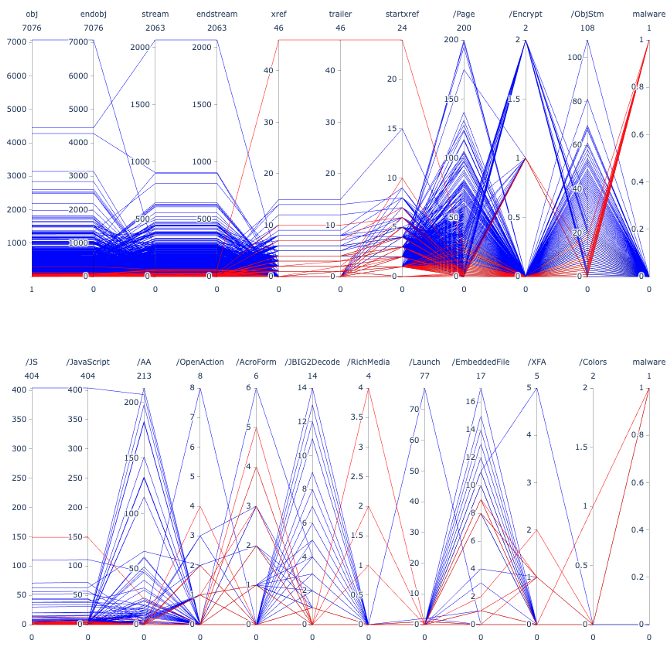
\includegraphics[width=\x\linewidth]{parallel_coords.png}
	\caption{The parallel plot highlights the difference between the features of Benign PDFs (Blue) and Malicious PDFs (Red)}
	\label{fig:parallel}
	\vspace{-5mm}
\end{figure}

\subsubsection{Model Validation}
We statically split the dataset in Train and Test using a stratified approach supplied by the \texttt{sklearn} library \cite{scikit-learn}. The Training Set, which consists of 80\% of the samples, is used to train and validate the models with a k-fold cross validation approach. The Test Set, which consists of 20\% of the entire dataset, is used to make final considerations about the performance of the models trained with the best parameters/hyperparameters.
To evaluate our models, we used two metrics: the False Negative Rate (FNR) and the Accuracy defined as:
\begin{center}
	$FNR = \frac{FN}{FN + TP} \quad Accuracy = \frac{TP+TN}{TP+TN+FP+FN}$
\end{center}
We aimed to minimize the FNR, as False Negatives (Malicious PDFs classified as Benign) can be particularly damaging in this context.
At the same time, we also took into consideration the value of the Accuracy, as the penalization of False Negative errors should not result in an excessively high number of False Positives that may lead to unnecessary alerts.

%%# SVM #%%
\section{Support vector machines}
\label{sec:svm}
% Intro that motivates why we use SVM (citing papers of \ref{sec:relatedwork})
Support Vector Machines are linear classifiers that look for maximum margin separation hyperplanes.
The soft margin SVM problem adds a penalty term $C\sum_{i=1}^{n}\xi_i$ to the hard margin SVM to relax the constraint of having points inside the margin. The hyperparameter $C$ is meant to define the strength of this penalization.
\subsection{Linear SVM}
% Few words about the linear SVM
We implemented a linear SVM classifier using the \texttt{sklearn} library(\cite{scikit-learn}). The samples $x_i$ are features vectors of $21$ elements (the ones extracted from PDFiD).

\subsubsection{Experiments}
% Results obtained with the linear SVM (plots)
We have cross-validated the linear model by trying $10$ different values for the $C$ hyperparameter in the range $[10^{-6}, 10]$. As explained in section \ref{sec:datasetsandfeatures} we optimized for the False Negative Rate (FNR) with the constraint of obtaining a high accuracy anyway.

\begin{figure}[ht!]
	\centering
	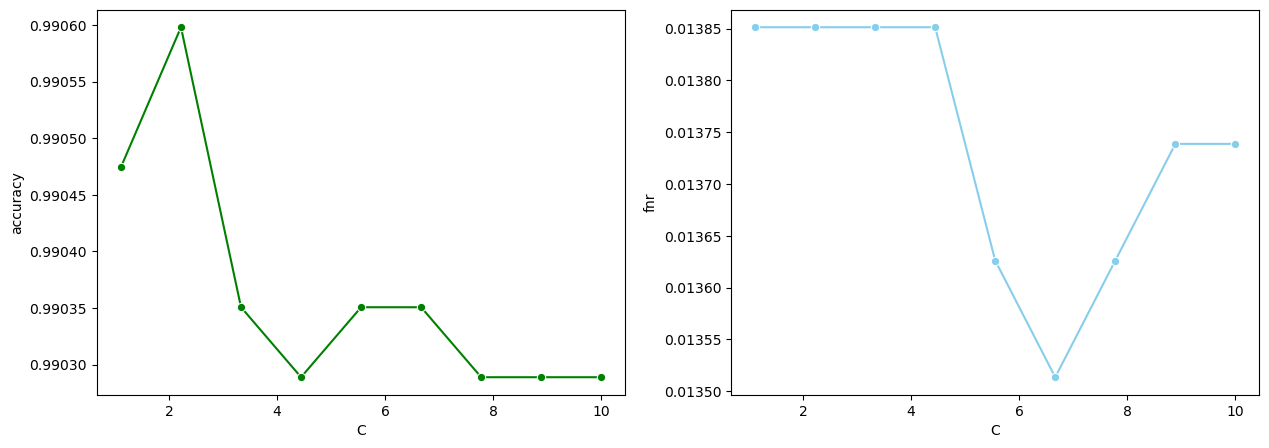
\includegraphics[width=\x\linewidth]{linear_svm_accuracy_fnr.png}
	\caption{The plots show how the accuracy (left) and the FNR (right) change when the value of $C$ hyperparameter changes}
	\label{fig:linearsvm}
\end{figure}

% comments on linear SVM
The plot in Figure \ref{fig:linearsvm} shows that the variations in terms of Accuracy and FNR when different values of $C$ are used to train the linear SVM are not that evident. Here the results obtained with $C=10^{-6}$ where not reported because of the significatively worse results ($88.67\%$ of Accuracy and $2.94\%$ of FNR). \\

\begin{table}[ht!]
	\centering
	{\small
		\begin{tabular}{|l|l|l|}
			\hline
			\textbf{C} & \textbf{Accuracy} & \textbf{FNR} \\ \hline
			2.22       & 99.06\%           & 1.38\%       \\ \hline
			6.67       & 99.03\%           & 1.35\%       \\ \hline
		\end{tabular}
	}
	\caption{Best model parameters for Linear SVM}
	\vspace{-6mm}
\end{table}

Optimizing for the FNR the hyperparameter we have selected is $C=6.67$.
\subsection{Kernel SVM}
% Why SVM are good: kernels
What it makes the SVM particularly powerful is the way the dual problem is defined becuase it allows to easily introduce a kernel function to express the problem in a higher dimensional features space. Thus, we implemented a Radial Basis Function (RBF) kernel that is defined as:
\begin{center}
	$k(x,y) = e^{-\gamma||x-y||^2}$
\end{center}

\subsubsection{Experiments}
\label{sub:expsvm}
% Results obtained with the RBF kernel SVM (plots)
The cross-validation of the model took into account two different hyperparameters ($\gamma$ for the RBF kernel and $C$ for the dual SVM problem).
This time we exploited a grid search k-fold cross validation that makes use of the CV to train the model with each possible combinations of hyperparameters. The hyperparameters values we tried are:
\begin{itemize}
	\item $\gamma$: 10 values in $[10^{-6}, 1]$
	\item $C$: 10 values in $[10^{-6}, 10]$
\end{itemize}
We investigated the influence of both hyperparameters. What it is not displayed and analyzed in the plots is what happens with $C=10^{-6}$ and $\gamma=10^{-6}$, parameters under which the classifier performs very poorly in terms of accuracy (around $54\%$) despite achieving a $FPR$ equal to $0\%$. However, this is not better than a dummy classifier that safely detects every PDF as malicious so it's not of interest in this project.

\begin{figure}[ht!]
	\centering
	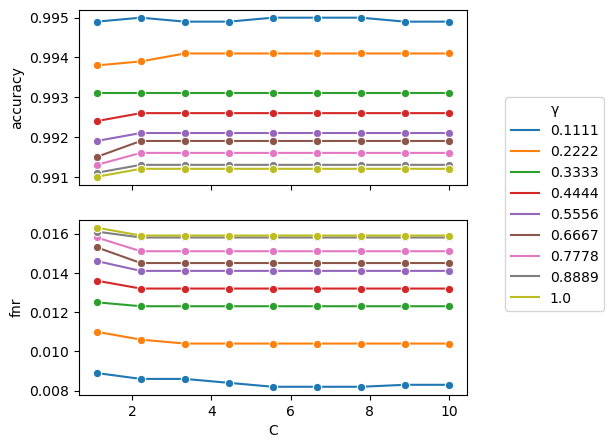
\includegraphics[width=\x\linewidth]{rbf_svm_gamma_accuracy_fnr.png}
	\caption{Accuracy (top) and FNR (bottom) when $\gamma$ (colored lines) changes and $C$ changes}
	\label{fig:rbfsvmgamma}
\end{figure}

In Figure \ref{fig:rbfsvmgamma} it's clear that smaller values of $\gamma$ lead to obtain better results both in terms of Accuracy and FNR. The $\gamma$ parameter of the RBF kernel controls its width and the shape of the decision boundary. A lower value of gamma means a larger, less concentrated kernel, which can lead to smoother decision boundaries.\newline
In contrast, the value of the $C$ hyperparameter has clearly less influence on the model than $\gamma$ as we can observe in Figure \ref{fig:rbfsvmgamma}. What it does is controlling the trade-off between the simplicity of the model (low bias, high variance) and the training error (low variance, high bias). A higher value of $C$ means a higher penalty for misclassification and the opposite for a lower value.
When $\gamma$ is sufficiently small the Accuracy reaches the best values and the same happens for the FNR.

Overall the best values we have found from cross validation are:
\begin{center}
	$C=5.56\quad\gamma=0.11 \quad Accuracy=99.50\% \quad FNR=0.82\%$
\end{center}

\subsection{Performances on Test Set}
Finally, given the best hyperparameters found in section \ref{sub:expsvm} we assessed the performances achieved on the Test Set.
\subsubsection{Linear SVM}
The obtained results are:
\begin{center}
	$C=6.67 \quad Accuracy=99.06\% \quad FNR=1.58\%$
\end{center}
The scores obtained are comparable with the ones achieved on the Training Set. Despite a smaller improvement in the Accuracy a slightly worse FNR has been obtained

\subsubsection{Kernel SVM}
The RBF SVM on the entire Test Set achieves these results:
\begin{center}
	$C=5.56 \quad \gamma=0.11 \quad Accuracy=99.73\% \quad FNR=0.36\%$
\end{center}
Here instead, we obtained better results over both Accuracy and FNR.
%%# DECISION TREE AND RANDOM FOREST #%%
\section{Decision tree and random forest}
\label{sec:tree}
\subsection{Decision Trees}
The Decision Tree is a classification technique in which predictions are made in a sequence of single-attribute tests.
Each internal node represents a test on an attribute, and each branch represents the outcome of the test. The paths from the root to the leaf nodes represent classification rules, and the leaf nodes represent class labels.
\subsubsection{Experiments}
\label{sub:tree}
We performed a k-fold cross validation with 5 folds in order to learn the best model parameters on the Training Set with more focus on $max\_depth$.
\begin{figure}[ht!]
	\centering
	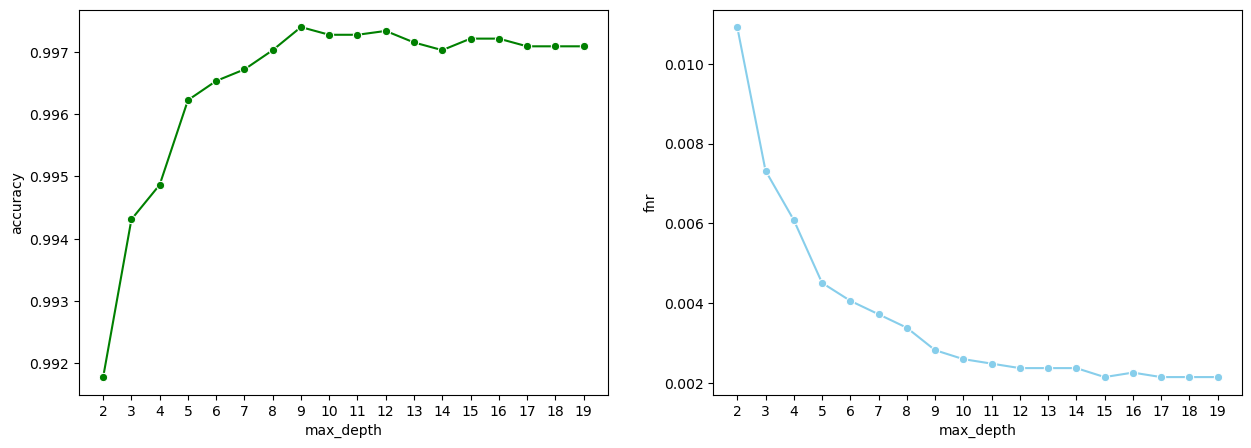
\includegraphics[width=\x\linewidth]{tree_accuracy_fnr.png}
	\caption{Accuracy (left) and FNR (right) when $max\_depth$ changes}
	\label{fig:treetrain}
\end{figure}
To summurize, the results we have obtained are reported in table \ref{tab:treetrain}.
\begin{table}[ht!]
	\centering
	{\small
		\begin{tabular}{|l|l|l|l|}
			\hline
			\textbf{max depth} & \textbf{Accuracy} & \textbf{FNR} \\ \hline
			15                 & 99.72\%           & 0.21\%       \\ \hline
			9                  & 99.74\%           & 0.28\%       \\ \hline
		\end{tabular}
		\caption{Decision Tree - Optimal depths from cross validation}
		\label{tab:treetrain}
		\vspace{-5mm}
	}
\end{table}
Despite the model achieves the best Accuracy with $max\_depth = 9$ we chose as best parameter the one that achieves the lowest $FNR$ that is $max\_depth = 15$.

\subsection{Random Forests}
Random Forests is an ensemble method that combines the predictions of multiple decision tree models to make a more accurate and stable predictions.
To train a Random Forests model, multiple Decision Trees are trained on different samples of the data and their predictions are combined. This helps to reduce overfitting and improve the model's generalization ability.

\subsubsection{Experiments}
\label{sub:randomforest}
We performed a k-fold cross validation with 5 folds in order to learn the best model parameters on the Training Set with more focus on $max\_depth$. The plot in \ref{fig:foresttrain} shows how both the Accuracy and the FNR improve as the depth of the tree increases. Choosing a not too high value of depth is crucial to avoid overfitting.

\begin{figure}[ht!]
	\centering
	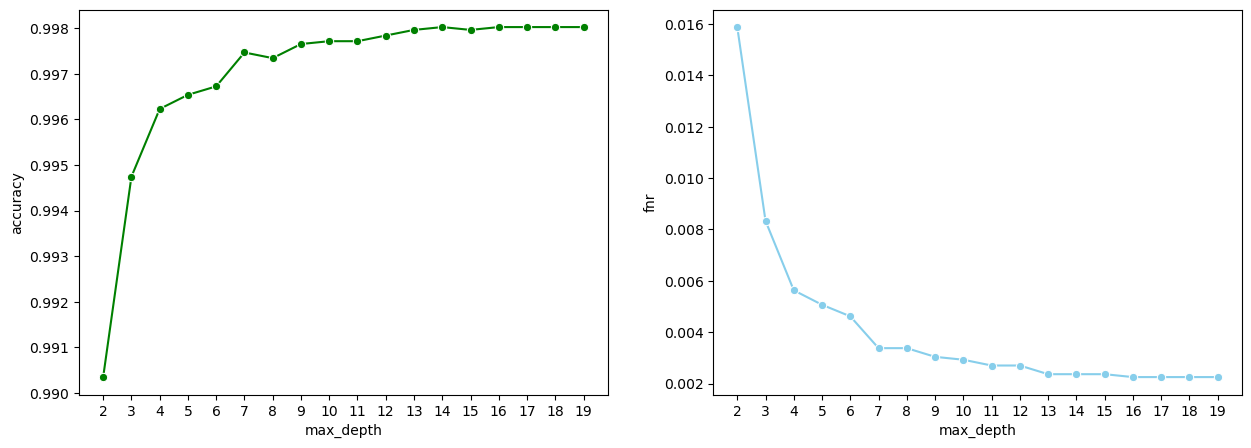
\includegraphics[width=\x\linewidth]{randomforest_accuracy_fnr.png}
	\caption{Accuracy (left) and FNR (right) when $max\_depth$ changes}
	\label{fig:foresttrain}
\end{figure}
The best obtained result is:
\begin{center}
	$max\_depth=16 \quad Accuracy=99.80\% \quad FNR=0.22\%$
\end{center}

\subsubsection{Performances on Test Set}
The results obtained on the Test Set of both Decision Trees and Random Forests using the best model parameters discussed in \ref{sub:tree} and \ref{sub:randomforest} are:
\begin{center}
	\textbf{Decision Trees}\\
	$max\_depth=15 \quad Accuracy=99.75\% \quad FNR=0.22\%$\\~\\
	\textbf{Random Forests}\\
	$max\_depth=16 \quad Accuracy=99.90\% \quad FNR=0.13\%$
\end{center}

%%# KNN #%%
\section{K-Nearest Neighbors}
\label{sec:knn}
K-Nearest Neighbors (KNN) works by identifying the $K$ number of training samples that are closest in distance to the input sample, and then assigning the input sample to the class of the majority of the $K$ nearest neighbors.
\subsection{Experiments}
We performed a k-fold cross-validation with 5 folds.
To determine the optimal value of $K$ (the number of nearest neighbors to consider), we conducted a grid search over a range of possible values ($K \in [1, 8]$).
\begin{figure}[ht!]
	\centering
	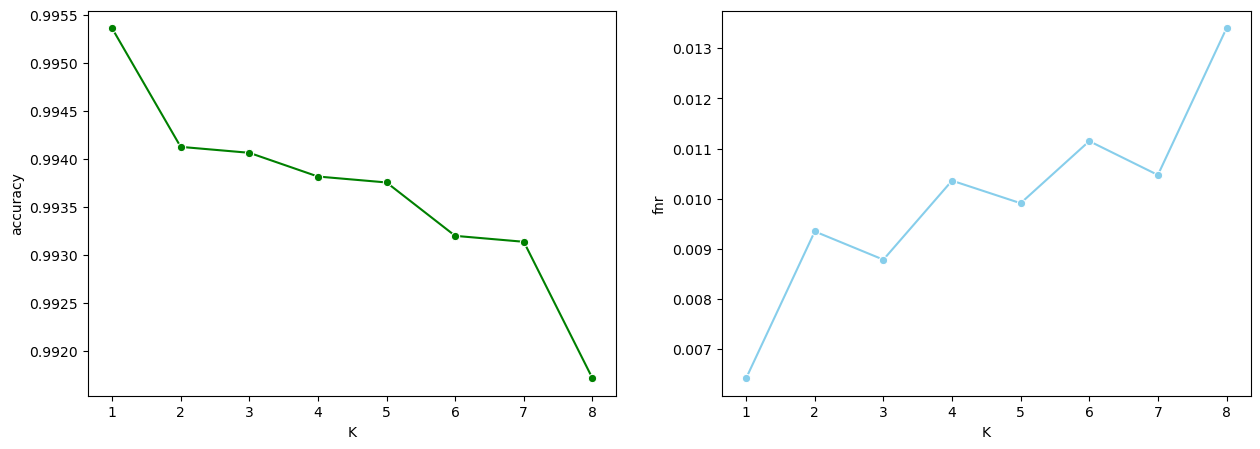
\includegraphics[width=\x\linewidth]{knn_accuracy_fnr.png}
	\caption{Accuracy (left) and FNR (right) when $K$ changes}
	\label{fig:knntrain}
\end{figure}
The results of this search shows, as expected, that the best performances were achieved with $K=1$. Since we have selected very discriminant features and we dispose of a large and diverse dataset, we expect that the possible overfitting effect will not be really high.
To visualize the effect of increasing $K$ on the performance of our model, we plotted in Figure \ref{fig:knntrain} the accuracy and FNR as a function of $K$. The performance of the model decreases slightly as $K$ increases. This is to be expected, as increasing $K$ allows the model to consider more neighbors, which can introduce more noise and reduce the model's ability to accurately classify samples. The best result obtained is:
\begin{center}
	$K=1 \quad Accuracy=99.67\% \quad FNR=0.82\%$
\end{center}

\subsection{Performances on Test Set}
The results on the Test Set are:
\begin{center}
	$K=1 \quad Accuracy=99.68\% \quad FNR=0.36\%$
\end{center}

We also obtained excellent results on the Test Set. We could explain the fact that $K=1$ is still the best model parameter by noticing that, despite the dataset is made of PDFs that are unique, PDFiD is able to extract such discriminant features that different PDFs result to be equal in terms of the extracted features vector. Having overlapped samples in the features space is really helpful for the way KNN classifies because the nearest neighbor of a test sample will probably consist in different overlapped samples, most of them belonging to the same class.
Our results demonstrate that KNN is an effective technique for detecting malicious PDFs, and that it can achieve high level performances with relatively little tuning.

%%# FINAL RESULTS #%%
\section{Final results}
\label{sec:finalresults}
We have summarized the results of all our classifiers in table \ref{tab:finalresults}.

The table shows that, as widely discussed in the previos sections, the model that achieves the best results is the Random Forests. Actually, all of them reach an impressively high accuracy and low FNR. This is also coherent with the results obtained in Corona et al. (\cite{maiorca_giacinto_corona_1970}) that proved Random Forests to be the best performing model. Also the other works cited achieve comparable results.
\begin{table}[ht!]
	\centering
	{\small
		\begin{tabular}{|c|cc|cc|}
			\hline
			                                                                        & \multicolumn{2}{c|}{\textit{\textbf{Train}}} & \multicolumn{2}{c|}{\textit{\textbf{Test}}}                                                         \\ \hline
			\textbf{Model}                                                          & \multicolumn{1}{c|}{\textbf{Accuracy}}       & \textbf{FNR}                                & \multicolumn{1}{c|}{\textbf{Accuracy}} & \textbf{FNR} \\ \hline
			\begin{tabular}[c]{@{}c@{}}Tree\\ $depth=15$\end{tabular}               & \multicolumn{1}{c|}{99.72\%}                 & 0.21\%                                      & \multicolumn{1}{c|}{99.75\%}           & 0.22\%       \\ \hline
			\begin{tabular}[c]{@{}c@{}}Forest\\ $depth=16$\end{tabular}             & \multicolumn{1}{c|}{99.80\%}                 & 0.22\%                                      & \multicolumn{1}{c|}{99.90\%}           & 0.13\%       \\ \hline
			\begin{tabular}[c]{@{}c@{}}KNN\\ $k=1$\end{tabular}                     & \multicolumn{1}{c|}{99.67\%}                 & 0.82\%                                      & \multicolumn{1}{c|}{99.68\%}           & 0.36\%       \\ \hline
			\begin{tabular}[c]{@{}c@{}}LSVM\\ $C=6.67$\end{tabular}                 & \multicolumn{1}{c|}{99.03\%}                 & 1.35\%                                      & \multicolumn{1}{c|}{99.06\%}           & 1.58\%       \\ \hline
			\begin{tabular}[c]{@{}c@{}}KSVM\\ $C=5.56$\\ $\gamma=0.11$\end{tabular} & \multicolumn{1}{c|}{99.50\%}                 & 0.82\%                                      & \multicolumn{1}{c|}{99.73\%}           & 0.36\%       \\ \hline
		\end{tabular}
	}
	\label{tab:finalresults}
	\caption{Overall results of all the models (LSVM: linear SVM, KSVM: RBF Kernel SVM). Results on Train are the ones obtained through k-fold cross validation}
	\vspace{-5mm}
\end{table}

Finally we also plotted the ROC curves for all the models. In Figure \ref{fig:roc} we can  confirm the results showed in table \ref{tab:finalresults}.
\begin{figure}[ht!]
	\centering
	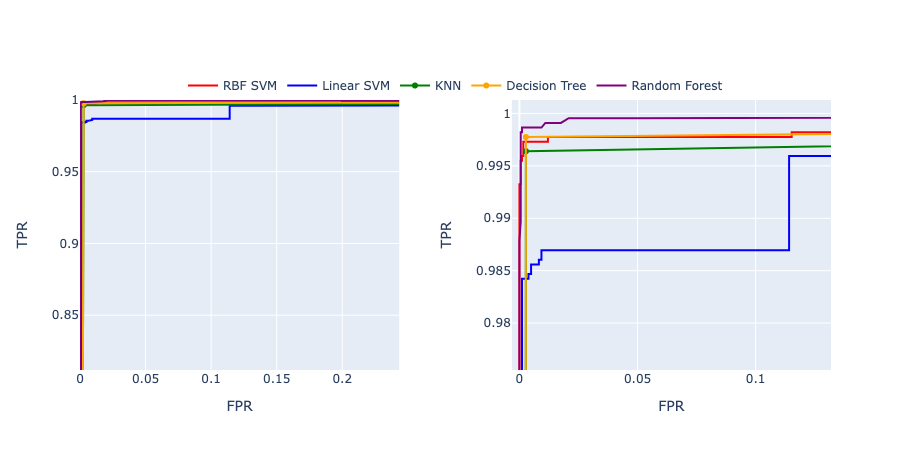
\includegraphics[width=\x\linewidth]{roc.png}
	\caption{ROC curve comparing all the different models. }
	\label{fig:roc}
\end{figure}

%%# ATTACKS TO CLASSIFIERS #%%
\section{Attacking the classifiers}
\label{sec:attacks}
In this section, we present two evasion attacks against the classifiers we built. We increased the number of objects in malicious PDFs so that they will be detected as Benign by the classifiers (still preserving their malicious behaviour). We operated in a condition in which the attacker is equipped with the Training Set, the type of classifier and the model parameters used to train it.
\subsection{Attack against SVM}
\label{subsec:svm}
We have studied an evasion attack based on the Gradient Descent algorithm following the idea of Cuan et al. in \cite{cuan_damien_delaplace_valois_2018}. Given
a feature vector $x$ characterizing a malicious PDF correctly classified, our goal is to find a $x'$ that will be detected as Benign. The constraint is that $x'$ is obtained with a minimal perturbation over $x$. The function to be minimized is the L1 distance between $x'$ and $x$:
\begin{center}
	$||x-x'|| = \sum_{i=1}^{d}x_i-x_i'$
\end{center}

The Gradient Descent attack converges to the minimum iteratively. Following the approach of Li et al. in \cite{li_liu_yan_yang_2022} the feature vector is moved in the negative direction of the gradient, that means that the Gradient Descent update step becomes:

\begin{center}
	$x_{t+1} = x_t - \mu_t\nabla_xf_{\Phi}(x_t)$
\end{center}
By recovering that $w = \nabla_x(w^Tx_t+w_0)$ for a linear SVM it can be derived that $w = \nabla_xf_{\Phi}(x_t)$ in a kernel SVM.
We obtained the expression for a RBF kernel SVM from the dual problem definition:
\begin{center}
	$\nabla_xf_{\Phi}(x_t) = \sum_{i \in SV}^{}\alpha_iz_i\nabla_xk(x_i,x_t)$
	where $\nabla_xk(x_i,x_t) = \nabla_{x_t}e^{-\gamma||x_i-x_t||^2}=-2\gamma\alpha_i z_i(x_i - x_t)e^{-\gamma||x_i-x_t||^2}$
\end{center}
To better get the idea behind the attack we trained a RBF SVM ($C=1$, $\gamma=0.1$) on the dataset preprocessing it with PCA (with 2 components) just to visualize it. In Figure \ref{fig:svmattack} a random malicious PDF is perturbated iteratively (using a learning rate for the Gradient Descent of $\mu=0.03$) and it is successfully attacked.
\begin{figure}[ht!]
	\centering
	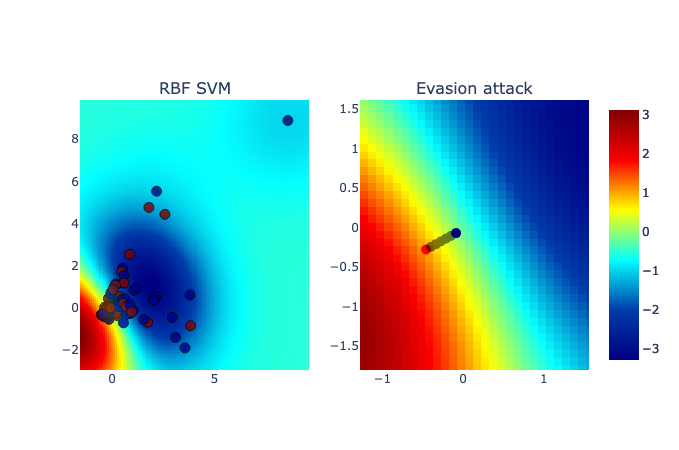
\includegraphics[width=\x\linewidth]{svmattack.png}
	\caption{Decision boundary of RBF SVM($C=1$, $\gamma=0.1$) on PCA=2 dataset (left), Gradient Descent attack on a random malicious PDF (right). (Blue: Benign, Red: malicious)}
	\label{fig:svmattack}
\end{figure}
We only inspected the working mechanism of this evasion attack by trying to successfully craft Benign PDFs from malicious ones.

\subsection{Attack against Decision Trees}
\label{subsec:tree}
We also investigated an attack against the Decision Trees classifier. Firstly we found a way to craft malicious PDFs that are detected as Benign (using a different approach with respect to the one used in \ref{subsec:svm} that is explained in the Pseudocode in \ref{alg:evasion}).
\begin{algorithm}
	{\footnotesize
		\caption{Evasion Attack}\label{alg:evasion}
		\begin{algorithmic}
			\Require Train DecisionTree using $X_{train}$
			\State $M \gets X_{train}[malicious]$
			\State $t \gets 50$
			\For{$m_i \in M$}
			\For{$feature_j \in m_i$}
			\While{$feature_j < t$}
			\State $feature_j \gets feature_j + 1$
			\State $m_i[j] \gets feature_j$
			\State $Benign \gets predict(m_i)$
			\If{$Benign$ is $True$}
			\State $break$  \Comment{PDF evaded}
			\EndIf
			\EndWhile
			\EndFor
			\Comment{PDF not evaded}
			\EndFor
		\end{algorithmic}
	}
\end{algorithm}

With a threshold $t=50$ we obtained a success rate of evasion attack on the Training Set equal to $91.28\%$.

\subsection{Adversarial Learning}
In order to improve the strenght of the Decision Trees classifier against the attack procedure in \ref{subsec:tree} we implemented a defense mechanism similar to what has been implemented by Cuan et al. in \cite{cuan_damien_delaplace_valois_2018}.
It is called Adversarial Learning and the algorithm is shown in Pseudocode \ref{alg:advlearn}.

\begin{algorithm}
	{\footnotesize
		\caption{Adversarial Learning}\label{alg:advlearn}
		\begin{algorithmic}
			\Require Train DecisionTree using $X_{train}$
			\State $t \gets 50$
			\State $X_{train}^{imp} \gets X_{train}$
			\State $M \gets X_{train}[malicious]$
			\While{$\#PDF evaded > 0$}
			\State $evaded,X_{train}^{evaded} \gets evade(M,t)$
			\If{$evaded$ is $True$}
			\State $X_{train}^{imp} \gets X_{train}^{imp} + X_{train}^{evaded}$
			\EndIf
			\State $train(X_{train}^{imp})$
			\EndWhile
		\end{algorithmic}
	}
\end{algorithm}

The results we obtain are overall satisfying because the classifier is able to defend perfectly against our evasion algrorithm.

\begin{figure}[ht!]
	\centering
	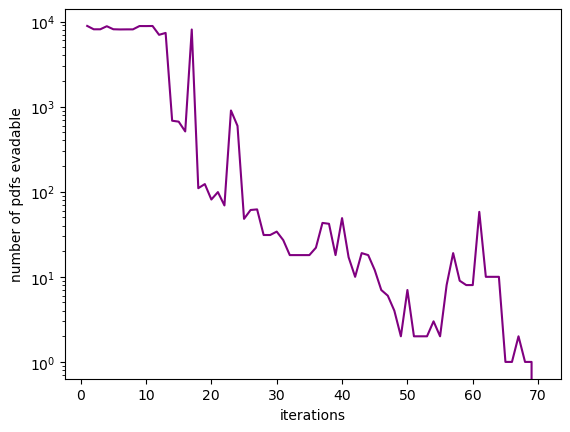
\includegraphics[width=\x\linewidth]{adv_learning.png}
	\caption{Adversarial Learning defense effectivness in different epochs: although the different spikes the number of evadable PDFs of Training Set reduces after each iteration}
	\label{fig:advlearn}
\end{figure}
The plot in Figure \ref{fig:advlearn} shows that the number of PDFs that can be evaded in the Training Set reaches $0$ at iteration $69$.\\
We can also see in Figure \ref{fig:improved} how the features of the improved dataset (the ones obtained adding the crafted PDFs to the original Training Dataset) have been modified to defend against this attack.

\begin{figure}[ht!]
	\centering
	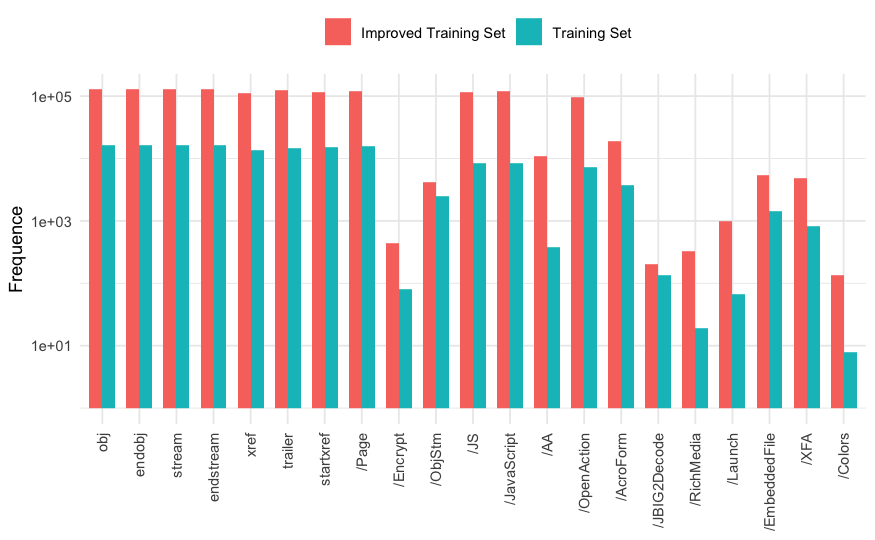
\includegraphics[width=\x\linewidth]{hist_train_improved.png}
	\caption{Difference of features frequencies between $X_{train}$ and $X_{train}^{imp}$ (logarithmic scale)}
	\label{fig:improved}
\end{figure}
%%# CONCLUSIONS #%%
\section{Conclusions and future works}
\label{sec:conclusions}
\paragraph{Classifiers}
To conclude, the model that performs better is the Random Forests both in terms of Accuracy and FNR. Comparable results are achieved by the others and the use of PDFiD makes all the algorithms efficient in detecting patters using the most discriminant features. Further improvement could be done in order to achieve even lower values of FNR. Dimensionality reduction techniques could be exploited toghether with other types of metrics that take into account both the Accuracy and the FNR.
\vspace{-10pt}
\paragraph{Evasion Attacks}
The evasion attack against the Decision Trees showed a really high success rate on the Training Set. We thus implemented the defense mechanism that proved to be very effective using Adversarial Learning. We could investigate more the size of the improved training dataset nedded to mitigate the attack.

%%# CONTRIBUTIONS #%%
\section{Contributions}
\label{sec:contributions}
These are the contributions of each member:
\begin{itemize}
	\item L. Ippolito worked on Decision Trees and Random Forests classifiers carefully exploring all the model parameters and the presence of overfitting.
	\item M. Picasso studied the KNN classifier to better understand the reason why $K=1$ is the best performing parameter.
	\item M. Rosso worked on SVM classifiers investigating the role of the different hyperparameters and the formulation of the dual soft margin SVM problem to be used in the evasion attacks.
\end{itemize}
We collaborated as a team both in the features extraction phase and on the choice of the model validation approach. After having assessed the performances of all the models we worked toghether on designing the evasion attacks algorithms and the countermeasueres.

%%%%%%%%%%%% Supplementary Methods %%%%%%%%%%%%
%\footnotesize
%\section*{Methods}

%%%%%%%%%%%%% Acknowledgements %%%%%%%%%%%%%
%\footnotesize
%\section*{Acknowledgements}

%%%%%%%%%%%%%%   Bibliography   %%%%%%%%%%%%%%
\normalsize
\bibliography{references}

%%%%%%%%%%%%  Supplementary Figures  %%%%%%%%%%%%
%\clearpage

%%%%%%%%%%%%%%%%   End   %%%%%%%%%%%%%%%%
%\end{multicols}  % Method B for two-column formatting (doesn't play well with line numbers), comment out if using method A
\end{document}
